\nicebox{
Change your exercise setup so that you set up a LAN with a computer behind the office computer, which you should then reach with the home computer. Check the function using a ping command. What must be considered?
}

\begin{figure}[H]
	\centering
	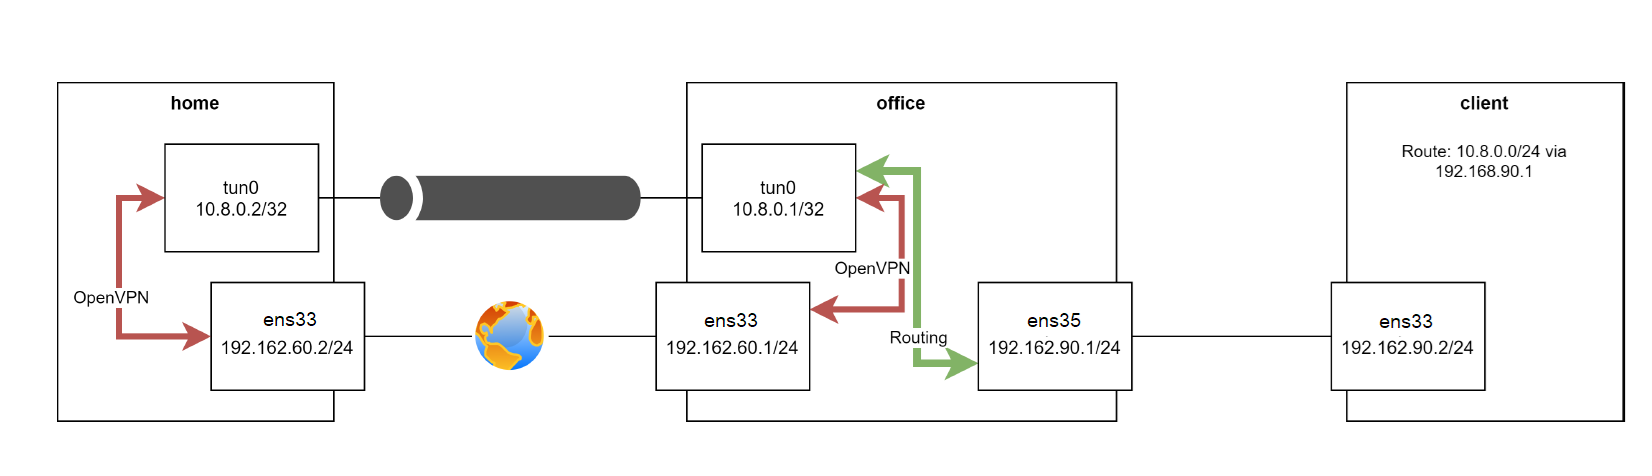
\includegraphics[width=1\linewidth]{Figures/home-office-lan.png}
	\caption{Home - Office - LAN Network}
\end{figure}

The static ip addresses were set with netplan again, but the LAN computer also needs a default route to the office computer, otherwise it won't know where to send the packets. Here is the config from the LAN computer:

\begin{minted}{yaml}
network:
  version: 2
  renderer: NetworkManager
  ethernets:
    ens33:
      dhcp4: no
      addresses:
       - 192.168.90.2/24
      routes:
       - to: default
         via: 192.168.90.1
         metric: 90
\end{minted}

For the home computer to send packets to the LAN computer, the office computer must forward the packets. This can be done by running the following command:

\begin{minted}{bash}
sudo sysctl -w net.ipv4.ip_forward=1
\end{minted}

The home computer also needs a route added in the home.conf file to reach the LAN computer:

\begin{minted}{console}
route 192.168.90.0 255.255.255.0 10.8.0.1
\end{minted}

This adds a route to 192.168.90.0/24 via 10.8.0.1, which is the office computer.

Using this configuration, the home computer can now ping the LAN computer:

\begin{minted}{console}
root@ntsi:/home/rdp# ping 192.168.90.1
PING 192.168.90.1 (192.168.90.1) 56(84) bytes of data.
64 bytes from 192.168.90.1: icmp_seq=1 ttl=64 time=4.84 ms
64 bytes from 192.168.90.1: icmp_seq=2 ttl=64 time=6.13 ms
\end{minted}

And the LAN computer can ping the home computer:

\begin{minted}{console}
root@ntsi:/home/rdp# ping 192.168.60.2
PING 192.168.60.2 (192.168.60.2) 56(84) bytes of data.
64 bytes from 192.168.60.2: icmp_seq=1 ttl=63 time=2.58 ms
64 bytes from 192.168.60.2: icmp_seq=2 ttl=63 time=3.41 ms
\end{minted}